% Author: Izaak Neutelings (March 2020)
% http://hyperphysics.phy-astr.gsu.edu/hbase/quantum/qangm.html
\documentclass[border=3pt,tikz]{standalone}
\usepackage{amsmath} % for \dfrac
\usepackage{mathabx} % for \Earth
\usepackage{bm} % \bm
\usepackage{physics}
\usepackage{tikz,pgfplots}
\usepackage[outline]{contour} % glow around text
\usetikzlibrary{angles,quotes} % for pic (angle labels)
\usetikzlibrary{calc}
\usetikzlibrary{decorations.markings}
\tikzset{>=latex} % for LaTeX arrow head
\contourlength{2.0pt}
\usepackage{xcolor}
\colorlet{Scol}{green!60!black}
\colorlet{veccol}{green!45!black}
\colorlet{myblue}{blue!60!black}
\colorlet{Bcol}{violet!90}
\tikzstyle{BField}=[->,thick,Bcol]
\tikzstyle{spin}=[->,very thick,Scol]
\tikzstyle{velocity}=[->,thick,vcol]
\tikzstyle{charge+}=[very thin,draw=black,top color=red!50,bottom color=red!90!black,shading angle=20,circle,inner sep=0.2]
\tikzstyle{charge-}=[very thin,draw=black,top color=blue!50,bottom color=blue!80,shading angle=20,circle,inner sep=0.2]
\tikzstyle{vector}=[->,thick,veccol]
\tikzset{
  BFieldLine/.style={thick,Bcol,decoration={markings,mark=at position #1 with {\arrow{latex}}},
                                 postaction={decorate}},
  BFieldLine/.default=0.5,
}


\begin{document}


% QUANTUM ANGULAR MOMENTUM
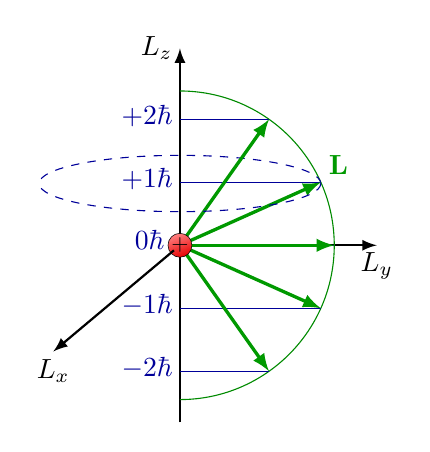
\begin{tikzpicture} %[z={(0,1)},y={(1,0)},x={(-0.5,0,-0.5)}]
  \def\zmax{2.5}
  \def\l{2}
  \def\h{0.8} %1.6/\l
  \def\R{(sqrt(\l*(\l+1))*\h)} % total angular momentum
  \def\M{1}
  \def\ang{asin(\M*\h/\R)}
  \def\Rx{sqrt(\R^2-(\M*\h)^2)}
  \def\Ry{0.2*\Rx}
  \coordinate (O) at (0,0);
  
  %\draw[->,thick] (O) --++ (-0.62*\zmax,-0.55*\zmax) node[below=-1] {$L_x$};
  \draw[->,thick] (O) --++ (\zmax,0) node[below=-1] {$L_y$};
  \draw[->,thick] (0,-0.9*\zmax) -- (0,\zmax) node[left=-1] {$L_z$};
  
  % CIRCLES
  \draw[Scol!90!black] (0,{\R}) arc (90:-90:{\R}); %,very thin
  \draw[dashed,myblue] ({\Rx},{\M*\h/sqrt(1+0.2^2)}) arc (0:180:{\Rx} and {\Ry});
  \foreach \m [evaluate={\y=\m*\h; \rx=sqrt(\R^2-(\m*\h)^2); \ry=0.2*\rx}] in {1,...,\l}{
    \draw[myblue] (0, \y) node[above=1,left=-1] {$+\m\hbar$} -- (\rx, \y);
    \draw[myblue] (0,-\y) node[above=1,left=-1] {$-\m\hbar$} -- (\rx,-\y);
    \draw[spin] (0,0) -- (\rx, \y);
    \draw[spin] (0,0) -- (\rx,-\y);
    %\draw[dashed,very thin] (\rx, \m*\h) arc (0:360:{\rx} and {\ry});
    %\draw[dashed,very thin] (\rx,-\m*\h) arc (0:360:{\rx} and {\ry});
  }
  \draw[myblue] (0,0) node[above=2,left=2] {$0\hbar$} -- ({\R},0);
  \draw[spin] (0,0) -- ({\R}, 0);
  \node[spin,above right=-1] at ({\Rx},{\M*\h}) {$\vb{L}$};
  %\draw[dashed,very thin] ({\Rx},\M*\h) arc (\ang:\ang+360:{\Rx} and {\Ry});
  %\draw[dashed,very thin] (0,{\M*\h/sqrt(1+0.2^2)}) ellipse ({\Rx} and {\Ry});
  \draw[dashed,myblue] ({\Rx},{\M*\h/sqrt(1+0.2^2)}) arc (0:-180:{\Rx} and {\Ry});
  %\draw[dashed,samples=100,smooth,variable=\t,domain=0:360]
  %  plot (0,{\R*cos(\t)},{\R*sin(\t)});
  \node[charge+,scale=0.8] (O) {$+$};
  \draw[->,thick] (-140:0.04*\zmax) --++ (-140:0.8*\zmax) node[below=-1] {$L_x$};
  
\end{tikzpicture}


% QUANTUM ANGULAR MOMENTUM - SPIN to scale
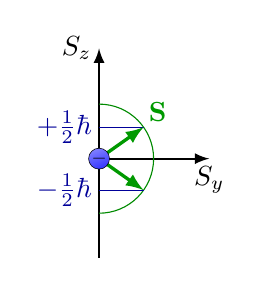
\begin{tikzpicture} %[z={(0,1)},y={(1,0)},x={(-0.5,0,-0.5)}]
  \def\zmax{1.4}
  \def\s{0.5}
  \def\h{0.8} %1.6/\l
  \def\R{(sqrt(\s*(\s+1))*\h)} % total angular momentum
  \def\M{0.5}
  \def\ang{asin(\M*\h/\R)}
  \def\Rx{sqrt(\R^2-(\M*\h)^2)}
  \def\Ry{0.2*\Rx}
  \coordinate (O) at (0,0);
  
  % AXES
  %\draw[->,thick] (-140:0.005*\zmax) --++ (-140:0.75*\zmax) node[below=-1] {$S_x$};
  \draw[->,thick] (O) --++ (\zmax,0) node[below=-1] {$S_y$};
  \draw[->,thick] (0,-0.9*\zmax) -- (0,\zmax) node[left=-1] {$S_z$};
  
  % CIRCLES
  \draw[Scol!90!black] (0,{\R}) arc (90:-90:{\R}); %,very thin
  %\draw[dashed,myblue] ({\Rx},{\M*\h/sqrt(1+0.2^2)}) arc (0:180:{\Rx} and {\Ry});
  \draw[myblue] (0,-\M*\h) node[left=-1,scale=1] {$-\frac{1}{2}\hbar$} --++ ({\Rx},0); %\contour{white}{
  \draw[myblue] (0,+\M*\h) node[left=-1,scale=1] {$+\frac{1}{2}\hbar$} --++ ({\Rx},0);
  \draw[spin] (0,0) -- ({\Rx},-\M*\h);
  \draw[spin] (0,0) -- ({\Rx}, \M*\h);
  \node[spin,above right=-2] at ({\Rx},{\M*\h}) {$\vb{S}$};
  %\draw[dashed,myblue] ({\Rx},{\M*\h/sqrt(1+0.2^2)}) arc (0:-180:{\Rx} and {\Ry});
  \node[charge-,scale=0.7] (O) {$-$};
  
\end{tikzpicture}


% QUANTUM ANGULAR MOMENTUM - SPIN enlarged
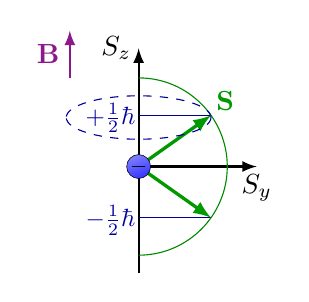
\begin{tikzpicture} %[z={(0,1)},y={(1,0)},x={(-0.5,0,-0.5)}]
  \def\zmax{1.5}
  \def\s{0.5}
  \def\h{1.3} %1.6/\l
  \def\R{(sqrt(\s*(\s+1))*\h)} % total angular momentum
  \def\M{0.5}
  \def\ang{asin(\M*\h/\R)}
  \def\Rx{sqrt(\R^2-(\M*\h)^2)}
  \def\Ry{0.3*\Rx}
  \coordinate (O) at (0,0);
  
  % AXES
  %\draw[->,thick] (-140:0.005*\zmax) --++ (-140:0.75*\zmax) node[below=-1] {$S_x$};
  \draw[->,thick] (O) --++ (\zmax,0) node[below=-1] {$S_y$};
  \draw[->,thick] (0,-0.9*\zmax) -- (0,\zmax) node[left=-1] {$S_z$};
  
  % CIRCLES
  \draw[Scol!90!black] (0,{\R}) arc (90:-90:{\R}); %,very thin
  \draw[dashed,myblue] ({\Rx},{\M*\h/sqrt(1+0.3^2)}) arc (0:180:{\Rx} and {\Ry});
  \draw[myblue] (0,-\M*\h) node[below=1,left=-2,scale=0.9] {$-\frac{1}{2}\hbar$} --++ ({\Rx},0); %\contour{white}{
  \draw[myblue] (0,+\M*\h) node[below=1,left=-2,scale=0.9] {$+\frac{1}{2}\hbar$} --++ ({\Rx},0);
  \draw[spin] (0,0) -- ({\Rx},-\M*\h);
  \draw[spin] (0,0) -- ({\Rx}, \M*\h);
  \node[spin,above right=-2] at ({\Rx},{\M*\h}) {$\vb{S}$};
  \draw[dashed,myblue] ({\Rx},{\M*\h/sqrt(1+0.3^2)}) arc (0:-180:{\Rx} and {\Ry});
  \node[charge-,scale=0.8] (O) {$-$};
  
  % B FIELD
  \draw[BField] ({-0.95*\Rx},0.75*\zmax) --++ (0,0.4*\zmax) node[midway,left] {$\vb{B}$};
  %\draw[BFieldLine] ({-1.2*\Rx},-1.2*\zmax) -- ({-1.2*\Rx},1.2*\zmax);
  %\draw[BFieldLine] ( 1.2*\zmax,-1.2*\zmax) -- ( 1.2*\zmax,1.2*\zmax);
  
\end{tikzpicture}


\end{document}
